\documentclass[12pt]{article}
\usepackage[margin=1in]{geometry}
\usepackage{amsmath, amssymb}
\usepackage{graphicx}
\usepackage{booktabs}
\usepackage{hyperref}
\usepackage{caption}
\usepackage{subcaption}
\usepackage{float}
\usepackage{parskip}
\graphicspath{{../figures/}}

\title{Two-Type Branching Process:\\
       Single-Pool and Parallel-Splitting Dynamics,\\
       and Estimation of Division Rates}
\author{}
\date{}

\begin{document}
\maketitle
%\tableofcontents
%\bigskip

% ─────────────────────────────────────────────────────────────────────────────
\section{Model Description}
\label{sec:model}

We simulate a two-type continuous-time branching process with cell types $X$
and $Y$.  Each cell divides independently and exponentially:

\begin{align}
  X \to X + X & \quad \text{rate } a \text{ per } X \text{ cell,} \\
  X \to X + Y & \quad \text{rate } b \text{ per } X \text{ cell,} \\
  Y \to Y + X & \quad \text{rate } c \text{ per } Y \text{ cell,} \\
  Y \to Y + Y & \quad \text{rate } d \text{ per } Y \text{ cell.}
\end{align}

Each division event creates exactly one new cell of the appropriate type;
the parent cell is not removed.  All four Poisson clocks are independent.
Events are sampled exactly using the Gillespie
algorithm~\cite{gillespie1977,gillespie1976}: at each step the time to the
next event is drawn from an exponential distribution with rate equal to the
total propensity, and the event type is chosen proportionally to the
individual propensities.

Throughout this analysis the parameters are fixed at
$a = 0.5$, $b = 0.1$, $c = 0.05$, $d = 0.4$, with initial condition
$n_X(0) = 1$, $n_Y(0) = 0$.  The process is stopped when the \emph{total}
cell count across all pools exceeds $N = 1000$.

\subsection{Theoretical long-run composition}

The mean dynamics satisfy
\[
  \frac{d}{dt}\begin{pmatrix}X\\Y\end{pmatrix}
  = \underbrace{\begin{pmatrix}a & c \\ b & d\end{pmatrix}}_{A}
    \begin{pmatrix}X\\Y\end{pmatrix}.
\]

The dominant eigenvalue of $A$ determines the exponential growth rate and
the corresponding eigenvector determines the long-run composition:

\[
  \lambda_1
  = \frac{(a+d) + \sqrt{(a-d)^2 + 4bc}}{2}
  = \frac{0.9 + \sqrt{0.03}}{2}
  \approx 0.537.
\]

The stable-composition eigenvector satisfies
$(A - \lambda_1 I)\mathbf{v} = 0$, giving

\[
  \frac{Y}{X}
  = \frac{\lambda_1 - a}{c}
  = \frac{0.037}{0.05}
  \approx 0.732,
  \qquad
  \frac{X}{X+Y}
  \approx 0.578.
\]

These values are the theoretical equilibrium targets regardless of initial
conditions.


% ─────────────────────────────────────────────────────────────────────────────
\subsection{Theoretical Variance of the Two Ratios}
\label{sec:variance}

\subsubsection{Moment equations for a single pool}

Because every cell divides independently, the process is a \emph{multi-type
linear birth process} and its moment equations can be derived from the master
equation.  Define, for a pool starting from a single type-$X$ founder:
\[
\mu_X(t) = E[X(t)], \quad \mu_Y(t) = E[Y(t)],
\]
\[
\sigma_{XX}(t) = \operatorname{Var}(X(t)), \quad
\sigma_{YY}(t) = \operatorname{Var}(Y(t)), \quad
\sigma_{XY}(t) = \operatorname{Cov}(X(t), Y(t)).
\]

The first moments satisfy
\begin{equation}
	\frac{d}{dt}\begin{pmatrix}\mu_X\\\mu_Y\end{pmatrix}
	= A\begin{pmatrix}\mu_X\\\mu_Y\end{pmatrix},
	\qquad A = \begin{pmatrix}a & c \\ b & d\end{pmatrix},
	\label{eq:mean_ode}
\end{equation}
so $(\mu_X(t),\mu_Y(t))^{\top} = e^{At}(1,0)^{\top}$.

Applying the generator to $X^2$, $XY$, and $Y^2$ and subtracting the square
of the mean yields the \emph{second central moment ODE system}:
\begin{align}
	\frac{d\sigma_{XX}}{dt} &= 2a\,\sigma_{XX} + 2c\,\sigma_{XY}
	+ (a\mu_X + c\mu_Y), \label{eq:sxx}\\
	\frac{d\sigma_{XY}}{dt} &= b\,\sigma_{XX} + (a+d)\,\sigma_{XY}
	+ c\,\sigma_{YY}, \label{eq:sxy}\\
	\frac{d\sigma_{YY}}{dt} &= 2b\,\sigma_{XY} + 2d\,\sigma_{YY}
	+ (b\mu_X + d\mu_Y), \label{eq:syy}
\end{align}
with initial conditions $\sigma_{XX}(0)=\sigma_{XY}(0)=\sigma_{YY}(0)=0$.
This is a \emph{linear} system driven by $(\mu_X,\mu_Y)$, so it can be
integrated exactly (e.g.\ via \texttt{scipy.integrate.odeint}).

\subsubsection{Delta method for the ratio variances}

Let $\alpha = \mu_X/(\mu_X+\mu_Y)$, $\beta = \mu_Y/(\mu_X+\mu_Y)$,
and $r = \mu_Y/\mu_X$.  Applying the delta method to the two ratios:

\begin{equation}
	\operatorname{Var}\!\left(\frac{X}{X+Y}\right)
	\approx
	\frac{\beta^2\,\sigma_{XX} + \alpha^2\,\sigma_{YY}
		- 2\alpha\beta\,\sigma_{XY}}{(\mu_X+\mu_Y)^2},
	\label{eq:var_r1}
\end{equation}

\begin{equation}
	\operatorname{Var}\!\left(\frac{Y}{X}\right)
	\approx
	\frac{r^2\,\sigma_{XX} + \sigma_{YY} - 2r\,\sigma_{XY}}{\mu_X^2}.
	\label{eq:var_r2}
\end{equation}

Both approximations are first-order and accurate when the population is large
relative to its standard deviation.

\subsubsection{Long-run behavior: spectral gap and concentration}

The homogeneous part of the second-moment system \eqref{eq:sxx}--\eqref{eq:syy}
has eigenvalues $\{2\lambda_1,\; \lambda_1+\lambda_2,\; 2\lambda_2\}$.
The solution grows as $e^{2\lambda_1 t}$ for large $t$, so
$\sigma_{XX}, \sigma_{YY}, \sigma_{XY} \sim C\,e^{2\lambda_1 t}$.
At the same time $\mu_X, \mu_Y \sim C' e^{\lambda_1 t}$, and hence
$(\mu_X+\mu_Y)^2 \sim e^{2\lambda_1 t}$.

The high positive correlation between $X$ and $Y$ (both driven by the
same Malthusian martingale~\cite{kesten1966,athreya1972}
$W = \lim_{t\to\infty} e^{-\lambda_1 t}
\mathbf{u}^{\top}\mathbf{Z}(t)$) makes the numerator of
\eqref{eq:var_r1} grow \emph{slower} than $e^{2\lambda_1 t}$.
The correct large-$t$ result is
\begin{equation}
	\operatorname{Var}\!\left(\frac{X}{X+Y}\right)
	\;\sim\; K\,e^{-2\varepsilon t},
	\qquad \varepsilon = \lambda_1 - \lambda_2
	= \sqrt{(a-d)^2+4bc}
	\approx 0.173,
	\label{eq:var_asymp}
\end{equation}
with an analogous decay for $\operatorname{Var}(Y/X)$.
The variance therefore decays \emph{exponentially} at a rate equal to twice
the spectral gap $\varepsilon$.  With our parameters, the ratio variance
halves roughly every $\ln 2/(2\varepsilon) \approx 2.0$ time units.

\begin{figure}[H]
	\centering
	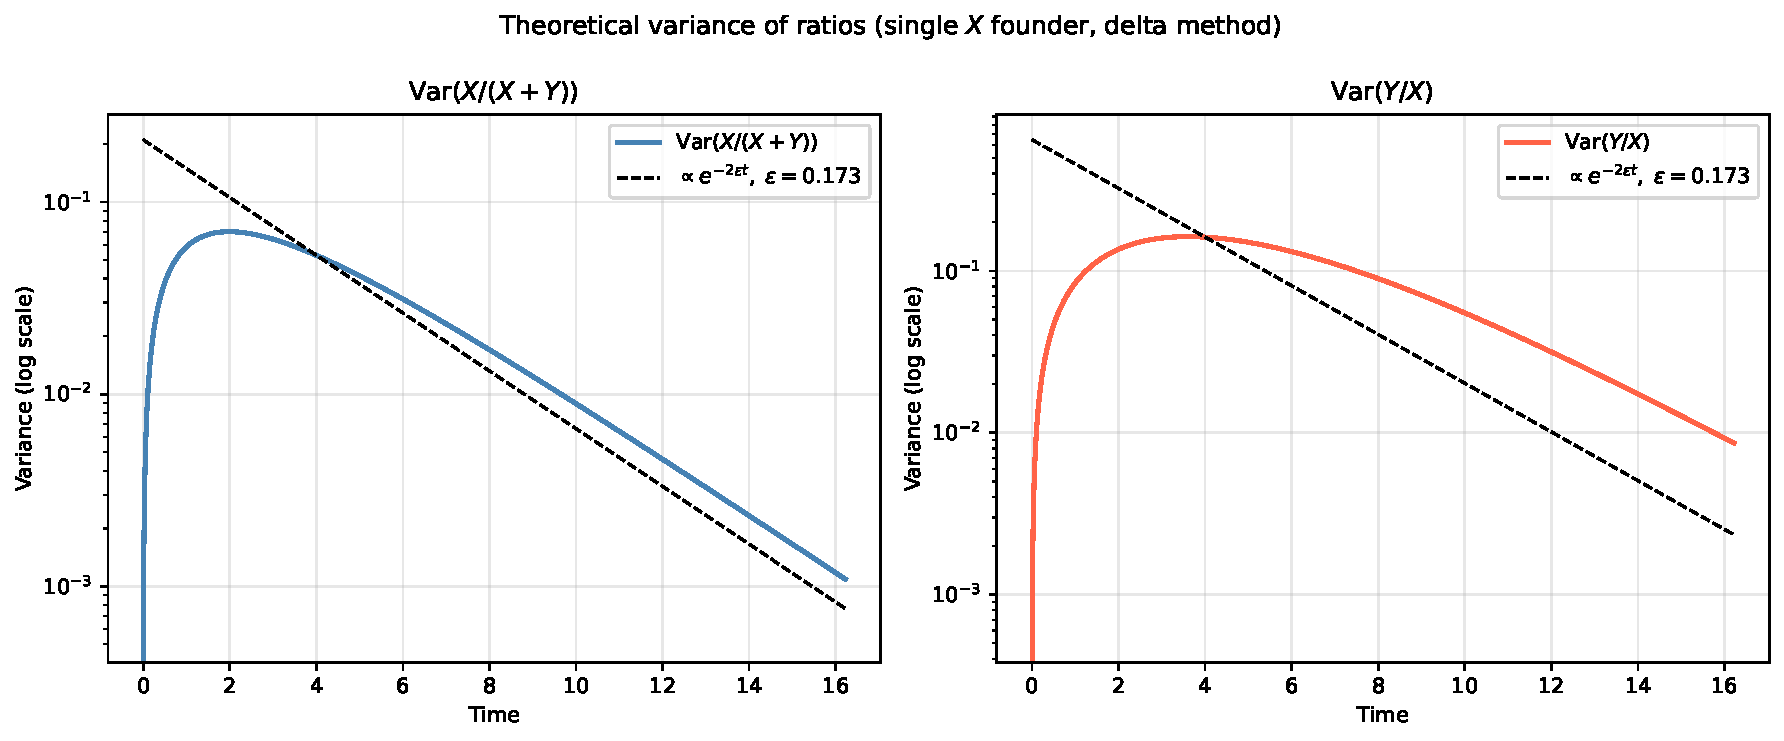
\includegraphics[width=0.9\textwidth]{fig_variance_theory.pdf}
	\caption{Theoretical variance curves for $X/(X+Y)$ (left) and $Y/X$
		(right), computed from the moment ODEs and delta method.  The
		dashed line marks the large-$t$ decay $\propto e^{-2\varepsilon t}$.}
	\label{fig:var_theory}
\end{figure}


% ─────────────────────────────────────────────────────────────────────────────
\section{Single-Pool Baseline}
\label{sec:single}

\begin{figure}[H]
  \centering
  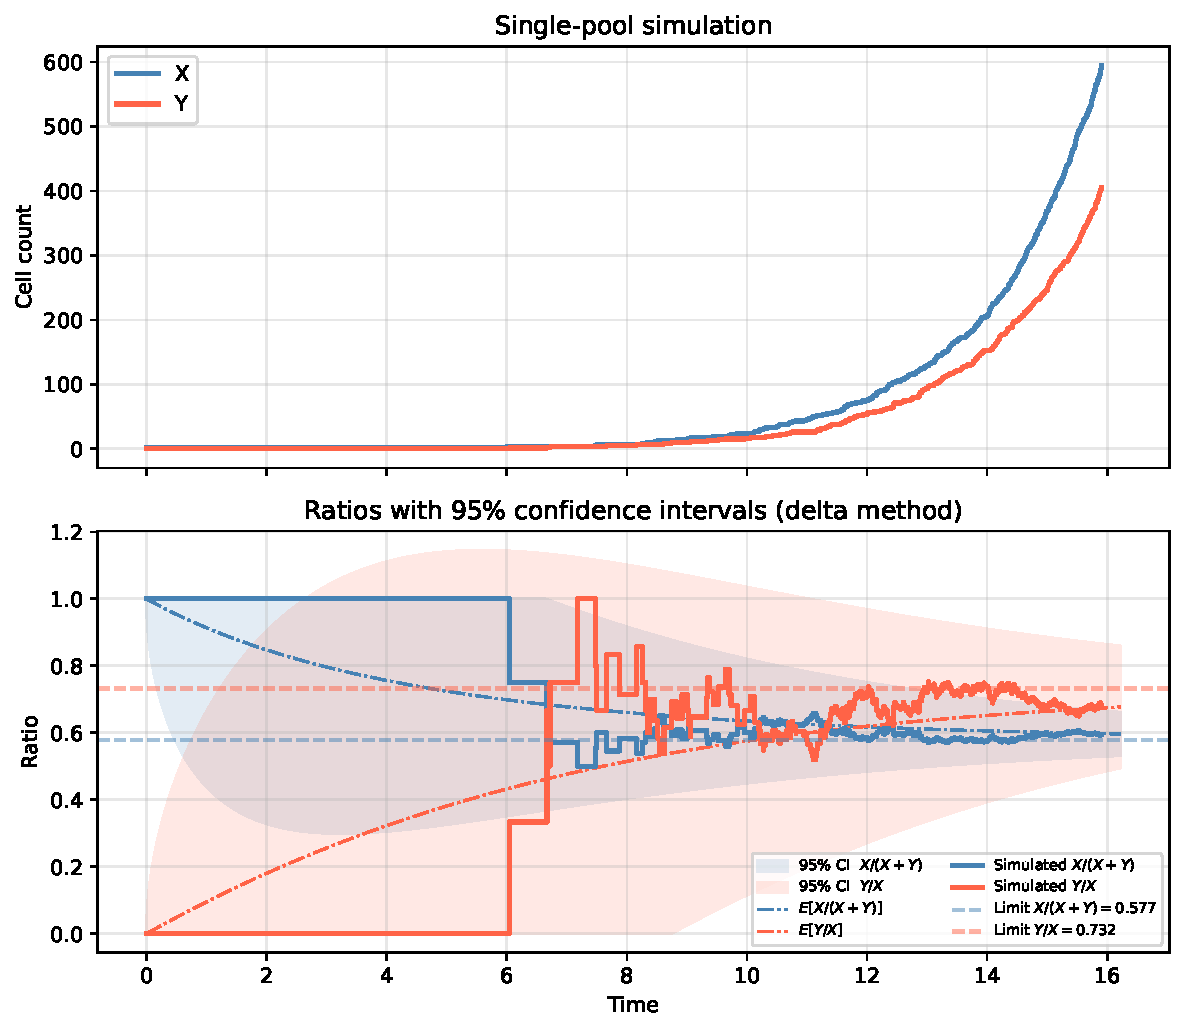
\includegraphics[width=0.85\textwidth]{fig_single.pdf}
  \caption{Single-pool Gillespie simulation~\cite{gillespie1977} ($N = 1000$,
           $n_X(0)=1$, $n_Y(0)=0$).  Top: counts of $X$ and $Y$ over time.
           Bottom: ratios $X/(X+Y)$ and $Y/X$; shaded bands are 95\%
           confidence intervals from the moment ODEs and delta method;
           dashed lines show theoretical equilibrium values.}
  \label{fig:single}
\end{figure}

Figure~\ref{fig:single} shows the baseline single-pool simulation.
Key observations:

\begin{itemize}
  \item \textbf{Exponential growth.}  Starting from a single $X$ cell the
        total population grows exponentially.  The growth is initially
        stochastic; once the population is large the law of large numbers
        removes visible fluctuations.

  \item \textbf{X initially dominates.}  Because the process starts as pure
        $X$ and $a \gg b$, $X$ cells accumulate rapidly before $Y$ cells
        appear via $X \to Y$ events.

  \item \textbf{Convergence of ratios.}  Both $X/(X+Y)$ and $Y/X$ converge
        toward the theoretical equilibrium ($\approx 0.578$ and
        $\approx 0.732$ respectively), illustrated by the dashed reference
        lines.  The convergence is not monotone because of stochastic
        fluctuations early in the process.

  \item \textbf{Long-run $Y/X < 1$.}  $Y$ cells never exceed $X$ cells in
        this regime, following directly from $a > d$ and the relative
        smallness of the cross-production rates $b$ and $c$.
\end{itemize}


% ─────────────────────────────────────────────────────────────────────────────
\section{Parallel Splitting}
\label{sec:parallel}

\subsection{Mechanism}

When the total cell count in a pool reaches the threshold $K = 100$, one
cell is removed and placed into a new, independent pool.  The removed cell
is of type $X$ with probability $p$ and type $Y$ with probability $1-p$.
The parent pool continues with $K - 1 = 99$ cells.

In \emph{parallel} mode all pools advance simultaneously on a shared,
real-valued time axis.  A global min-heap orders every pool's next potential
division event by its scheduled time; at each step the soonest event fires,
the affected pool is updated, and a new event is drawn from that pool.
All pools therefore coexist and grow concurrently.

Note that a split does not change the total cell count; only division events
do.  Therefore the global exponential growth rate $\lambda_1$ is unaffected
by $K$ and $p$; what changes is the \emph{composition} trajectory.

\subsection{Results: $K = 100$ — near-equilibrium regime}

\begin{figure}[H]
  \centering
  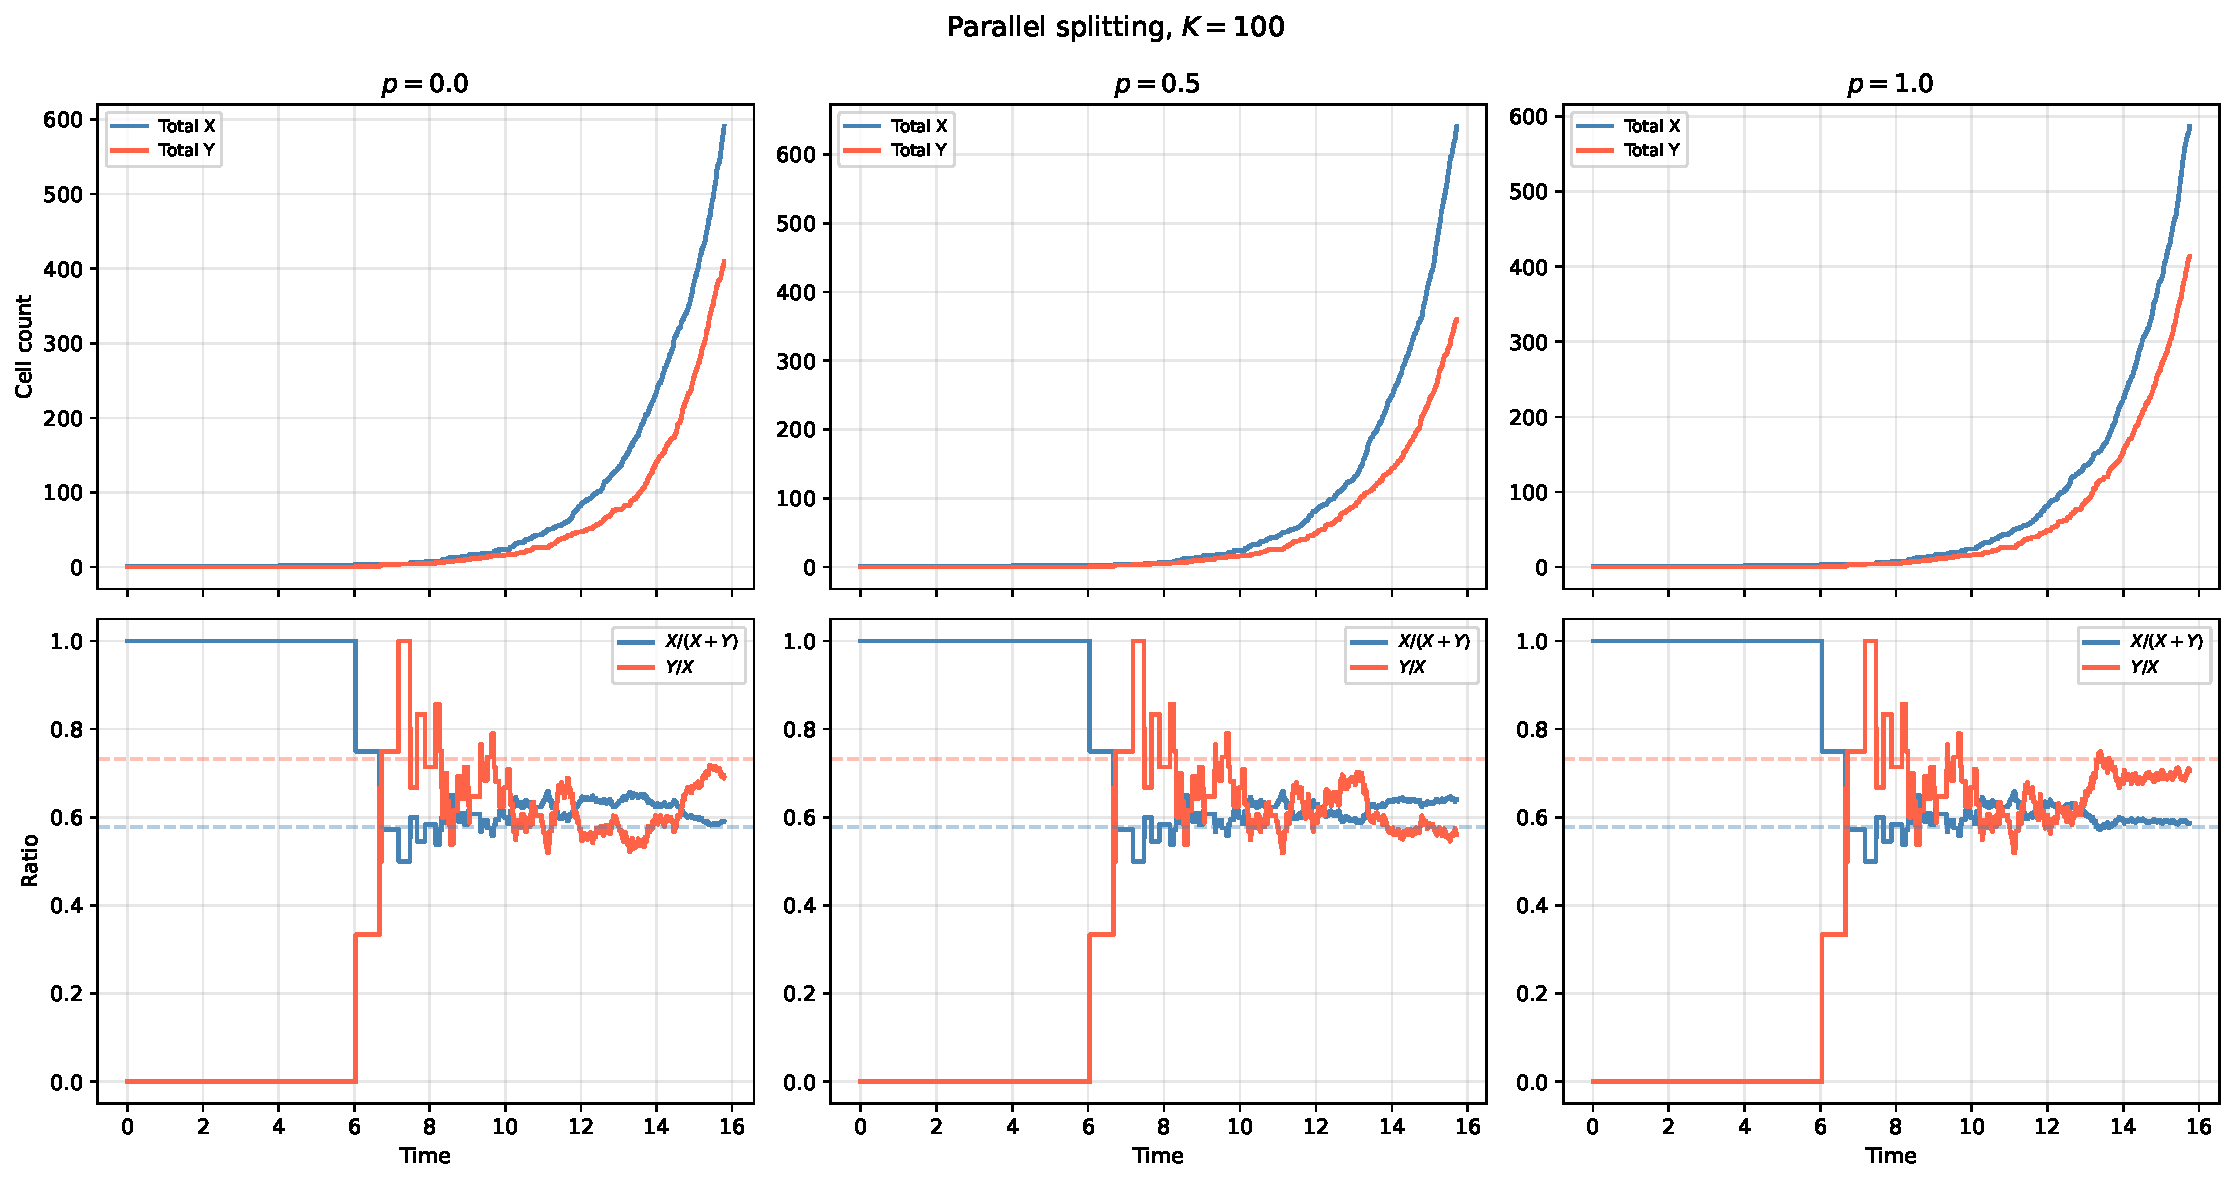
\includegraphics[width=\textwidth]{fig_par_K100.pdf}
  \caption{Parallel-mode split simulation with $K = 100$.  Columns:
           $p = 0$ (all splits seed a $Y$ cell), $p = 0.5$ (equal
           probability), $p = 1$ (all splits seed an $X$ cell).
           Top row: total $X$ and $Y$ counts across all pools.
           Bottom row: ratios $X/(X+Y)$ and $Y/X$; dashed lines mark
           theoretical equilibrium.}
  \label{fig:par_K100}
\end{figure}

Figure~\ref{fig:par_K100} shows the parallel splitting results for the
three extreme values of $p$.  A striking feature is the near
\emph{independence from $p$}: all three trajectories converge to values
close to the theoretical equilibrium $X/(X+Y) \approx 0.578$.

\paragraph{Why is parallel splitting robust to $p$?}
Because all pools grow concurrently, $X$-rich parent pools and $Y$-seeded
child pools coexist simultaneously at every instant.  Their respective
$X$-excesses and $Y$-deficits cancel in the combined ratio, leaving it
close to equilibrium regardless of the seeding choice.

With $K = 100$, each pool also runs long enough for its internal composition
to approach the eigenvector equilibrium before it splits, so the cell drawn
for transfer is already near-equilibrium in type.

\subsection{Results: $K = 20$ — founder-effect regime}

\begin{figure}[H]
  \centering
  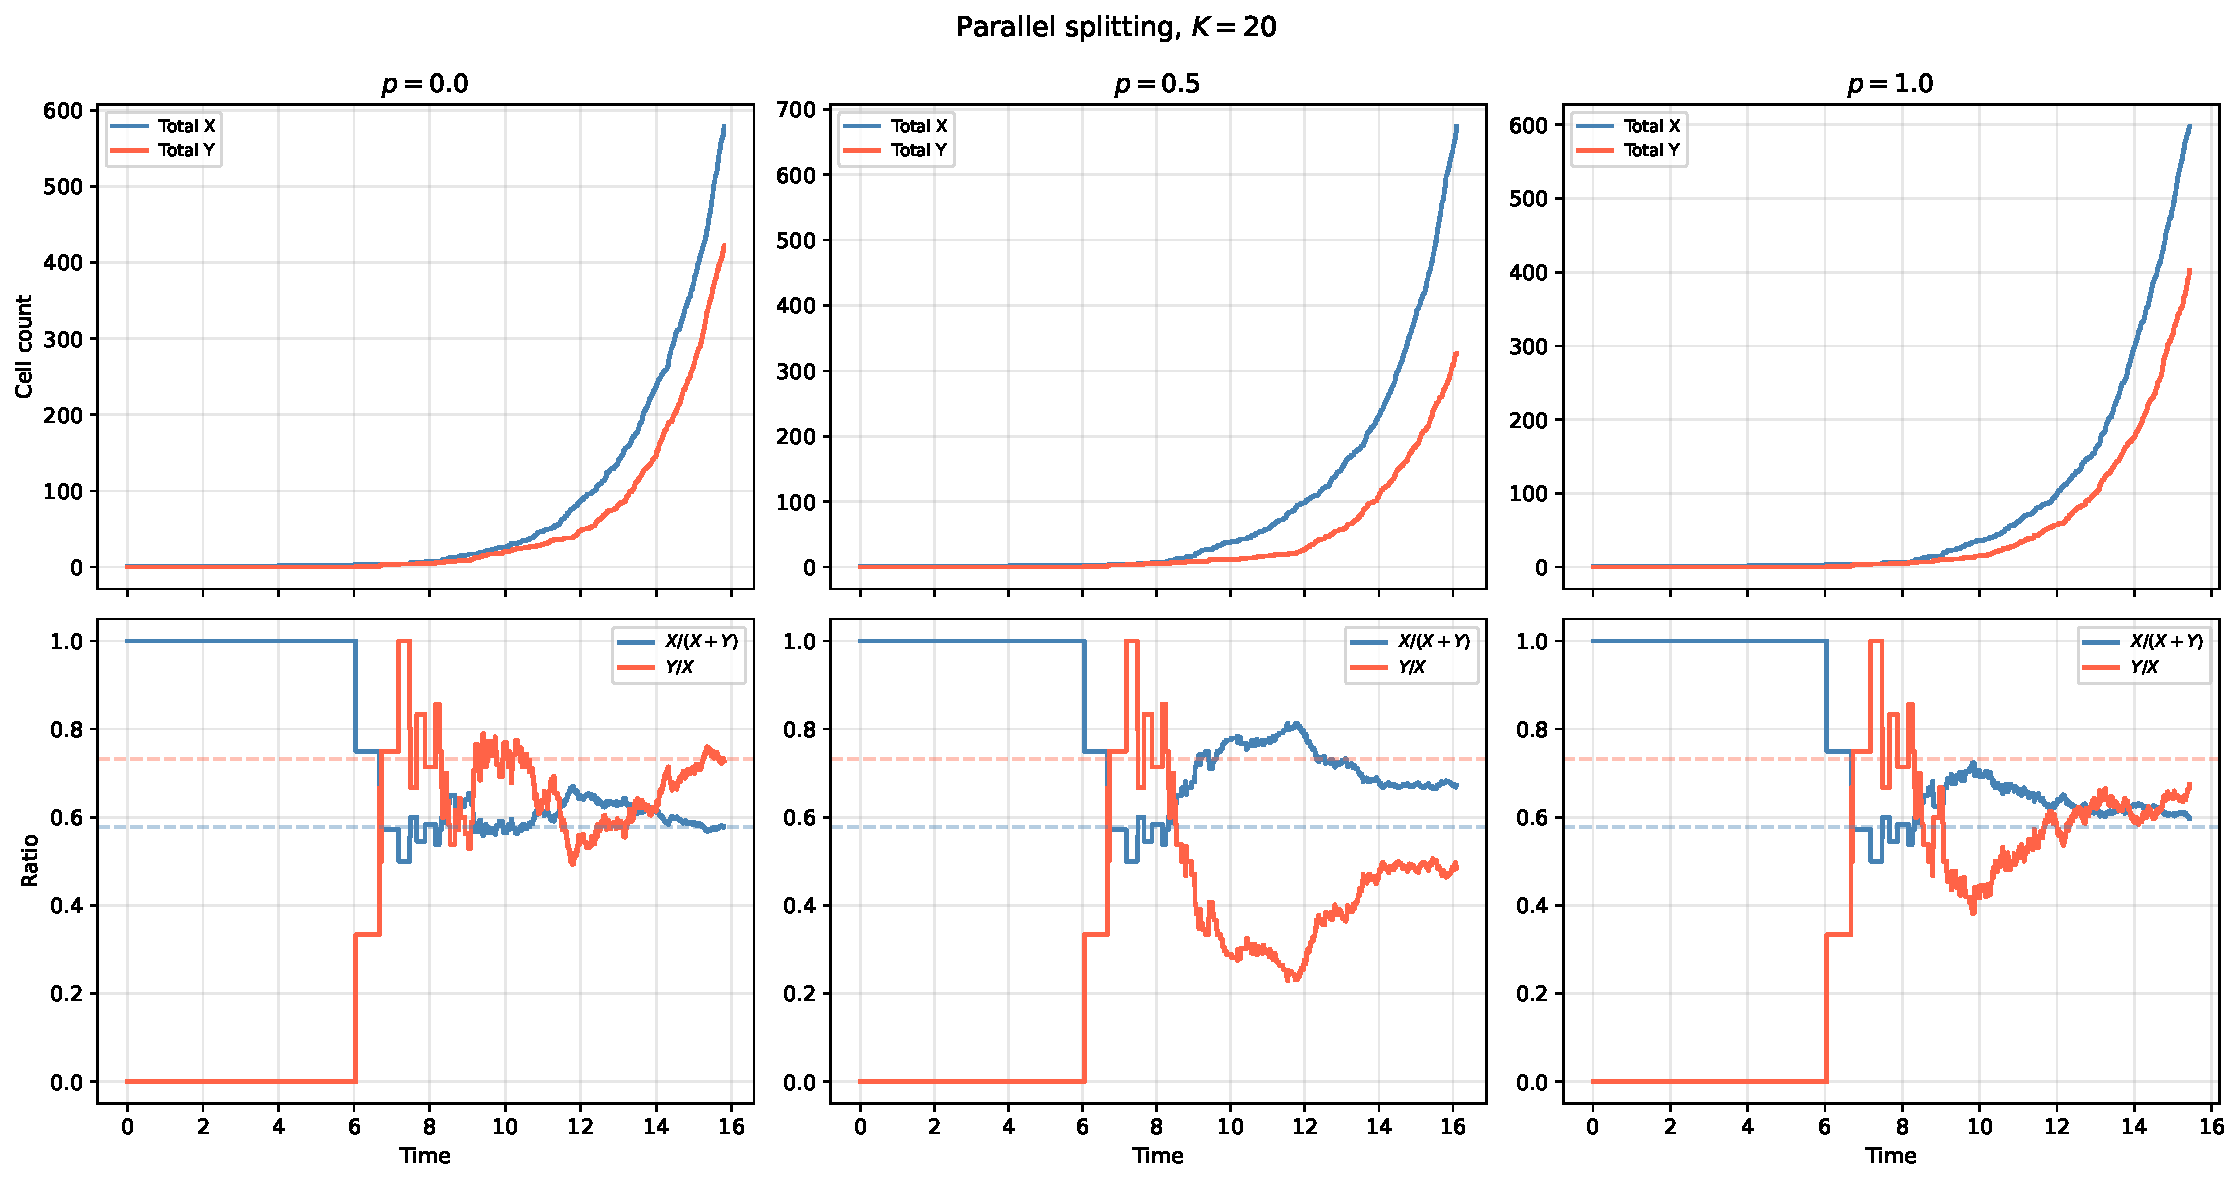
\includegraphics[width=\textwidth]{fig_par_K20.pdf}
  \caption{Parallel-mode split simulation with $K = 20$.  Layout identical
           to Figure~\ref{fig:par_K100}.  With smaller pools the ratios show
           stronger sensitivity to $p$ and larger transient fluctuations
           compared to the $K = 100$ case.}
  \label{fig:par_K20}
\end{figure}

Figure~\ref{fig:par_K20} repeats the experiment with $K = 20$, exposing the
regime in which pools are too small to equilibrate internally before splitting.
Two differences from the $K = 100$ case stand out.

\begin{itemize}
  \item \textbf{Higher sensitivity to $p$.}  With $K = 20$, a founder cell
        of type $Y$ has only 19 subsequent division opportunities before the
        pool splits.  Given the small cross-production rate $c = 0.05$, this
        is insufficient for the composition to approach the equilibrium
        eigenvector; $Y$-rich pools remain $Y$-rich.  The combined ratio
        therefore depends more strongly on $p$: the three columns of
        Figure~\ref{fig:par_K20} are visibly more separated than those of
        Figure~\ref{fig:par_K100}.

  \item \textbf{Larger transient fluctuations.}  With many small pools,
        each pool's founder type makes a larger fractional contribution to
        the combined ratio, so stochastic founder variation translates into
        more visible steps in the ratio trajectories.
\end{itemize}

The contrast between Figures~\ref{fig:par_K100} and~\ref{fig:par_K20}
illustrates the role of $K$ as a parameter controlling the trade-off between
\emph{mixing speed} (larger $K$ allows each pool to equilibrate internally)
and \emph{pool count} (smaller $K$ creates more pools, potentially improving
rate estimation as discussed in Section~\ref{sec:estimation}).


% ─────────────────────────────────────────────────────────────────────────────
\section{Comparison: Single Pool vs Parallel Splitting}
\label{sec:comparison}

Table~\ref{tab:summary} summarizes the two scenarios at $N = 1000$.

\begin{table}[H]
\centering
\caption{Final composition (averages over last 10\% of events).
         Theory: $X/(X+Y)\approx 0.578$, $Y/X\approx 0.732$.}
\label{tab:summary}
\begin{tabular}{lrrrrr}
\toprule
Scenario & Pools & $n_X$ & $n_Y$ & $X/(X+Y)$ & $Y/X$ \\
\midrule
Single pool              &   1  & 595 & 405 & 0.596 & 0.678 \\
\addlinespace
$K=100$, $p=0.0$  & 260  & 591 & 410 & 0.588 & 0.700 \\
$K=100$, $p=0.5$  & 248  & 641 & 360 & 0.641 & 0.560 \\
$K=100$, $p=1.0$  & 211  & 587 & 414 & 0.590 & 0.695 \\
\midrule
\multicolumn{4}{l}{\emph{Theory (equilibrium)}} & 0.578 & 0.732 \\
\bottomrule
\end{tabular}
\end{table}

\paragraph{Why are there so many pools?}
A naive estimate would give $N/K = 1000/100 = 10$ pools.  The actual count
($\sim\!210$--$260$) is far larger because the splitting mechanism creates a
cascade.  After the first pool grows from $1$ to $K = 100$ cells (requiring
$K-1 = 99$ divisions), it splits: one cell goes to a new child pool and the
parent retains $K-1 = 99$ cells.  The parent now needs only \emph{one} more
division to reach $K$ again and split a second time.  It therefore generates
a new child pool with approximately every subsequent division, acting as a
continuous source of single-cell founders.  As the simulation progresses,
child pools that themselves grow to size $K$ become additional sources,
amplifying the cascade further.  The result is that the number of pools
scales as $O(N)$ rather than $O(N/K)$; specifically, the pool count equals
$1 + (\text{total splits})$, where the total splits depend on how many
division events happen in pools already at size $K-1$.  With $N = 1000$ and
$K = 100$ this produces $\sim\!250$ pools, roughly $25\times$ the naive
estimate.

The following points summarize the key differences.

\begin{enumerate}
  \item \textbf{Growth shape.}  The single-pool simulation shows smooth
        near-exponential growth once the early stochastic phase passes.
        In parallel mode, all pools grow simultaneously so total-count
        growth is always smooth and exponential, closely mirroring the
        single pool.

  \item \textbf{Composition convergence.}  In the single pool both types
        always coexist and the composition drifts gradually toward equilibrium.
        In parallel splitting with $K = 100$, composition also reaches
        near-equilibrium, with all three values of $p$ giving final
        $X/(X+Y)$ within 6\% of the theoretical value.

  \item \textbf{Number of pools.}  Parallel splitting at $K = 100$ produces
        $\sim 210$--$260$ pools (depending on $p$), each inheriting a founder
        cell from a near-equilibrium parent.  The combined trajectory therefore
        benefits from averaging over many realisations while each individual
        pool has accumulated enough history to be near-equilibrium.

  \item \textbf{Variance of ratios.}  Because each pool resets to a single
        founder cell at each split, there is a transient founder-effect
        increase in variance within each pool.  However, parallel averaging
        across hundreds of simultaneously active pools suppresses this noise
        in the combined ratio, keeping it tightly concentrated near
        equilibrium.

  \item \textbf{Robustness to $p$.}  The parallel mode is nearly $p$-independent
        for $K = 100$: the final $X/(X+Y)$ ranges only from 0.588 to 0.641
        across all three $p$ values (Table~\ref{tab:summary}).%, which is a
        %much narrower range than would be seen in sequential mode.
\end{enumerate}


% ─────────────────────────────────────────────────────────────────────────────
\section{Estimation of Rate Parameters}
\label{sec:estimation}

So far the rates $a, b, c, d$ were treated as known.  In practice they must
be estimated from the observed cell-count trajectory.  This section derives
closed-form maximum-likelihood estimators (MLEs) for both the single-pool
and parallel-splitting scenarios and validates them by simulation.

\subsection{Log-likelihood and closed-form MLEs}

The process is a continuous-time Markov chain (CTMC) in which each $X$ cell
independently generates $X\!\to\!X{+}X$ events at rate $a$ and
$X\!\to\!X{+}Y$ events at rate $b$, while each $Y$ cell generates
$Y\!\to\!Y{+}X$ events at rate $c$ and $Y\!\to\!Y{+}Y$ events at rate $d$.
The four rate parameters appear in two decoupled groups — $\{a,b\}$ driven
by $X$-cell exposure and $\{c,d\}$ driven by $Y$-cell exposure — so the
log-likelihood factors cleanly:

\begin{equation}
  \ell(a,b,c,d)
  = n_a\log a + n_b\log b - (a+b)\Lambda_X
  + n_c\log c + n_d\log d - (c+d)\Lambda_Y,
  \label{eq:loglik}
\end{equation}

where:
\begin{itemize}
  \item $n_a$, $n_b$, $n_c$, $n_d$ are the observed counts of
        $X\!\to\!X{+}X$, $X\!\to\!X{+}Y$, $Y\!\to\!Y{+}X$, and
        $Y\!\to\!Y{+}Y$ events, respectively;
  \item $\Lambda_X = \int_0^T n_X(t)\,dt$ and
        $\Lambda_Y = \int_0^T n_Y(t)\,dt$ are the total \emph{cell-time
        exposures} of type $X$ and $Y$ over the observation window $[0,T]$.
\end{itemize}

Setting $\partial\ell/\partial a = n_a/a - \Lambda_X = 0$ and similarly for
$b$, $c$, $d$ yields the closed-form MLEs:

\begin{equation}
  \hat{a} = \frac{n_a}{\Lambda_X},\quad
  \hat{b} = \frac{n_b}{\Lambda_X},\quad
  \hat{c} = \frac{n_c}{\Lambda_Y},\quad
  \hat{d} = \frac{n_d}{\Lambda_Y}.
  \label{eq:mle}
\end{equation}

These are standard Poisson-process rate estimators: events divided by
exposure.  The second derivatives confirm $\ell$ is strictly concave in each
parameter, so \eqref{eq:mle} are global maxima.

\subsection{Single-pool estimator}

From the Gillespie trajectory $(t_0, t_1, \ldots, t_M;\, n_X(t_i),\, n_Y(t_i))$
the sufficient statistics are computed as:
\[
  \Lambda_X = \sum_{i=0}^{M-1} n_X(t_i)\,(t_{i+1}-t_i),
  \qquad
  \Lambda_Y = \sum_{i=0}^{M-1} n_Y(t_i)\,(t_{i+1}-t_i),
\]
and $n_a,\ldots,n_d$ are read directly from the event labels.
Because the simulation terminates \emph{exactly} at the $N$-th division
event, there is no missing tail interval: $t_M = T$ and $\Lambda_X,
\Lambda_Y$ are fully accounted for.  The plug-in estimator~\eqref{eq:mle}
is therefore straightforward to apply.

\subsection{Parallel splitting estimator}

For parallel splitting, $n_a,\ldots,n_d$ and $\Lambda_X, \Lambda_Y$ are
aggregated over all pools:
\[
  n_a = \sum_p n_a^{(p)}, \quad
  \Lambda_X = \sum_p \Lambda_X^{(p)}, \quad \text{etc.}
\]
Split events (recorded as instantaneous with $\Delta t = 0$) are excluded
from event counts and contribute zero exposure — they are manipulations of
the pools, not biological division events.

\paragraph{Tail correction.}
When the global simulation stops at time $T_{\mathrm{stop}}$ (the moment the
$N$-th total cell is produced), the pool that triggered termination is recorded
fully up to $T_{\mathrm{stop}}$.  All other pools, however, have a final
interval $[t^{(p)}_{\mathrm{last}},\, T_{\mathrm{stop}}]$ that is not yet
captured in their traces.  Omitting this interval \emph{understates}
$\Lambda_X$ and $\Lambda_Y$, inflating the rate estimates.

The corrected exposures are:
\begin{equation}
  \Lambda_X^{\mathrm{corr}}
  = \Lambda_X^{\mathrm{raw}}
  + \sum_{p} n_X^{(p)}\!\left(t^{(p)}_{\mathrm{last}}\right)
    \cdot \bigl(T_{\mathrm{stop}} - t^{(p)}_{\mathrm{last}}\bigr),
  \label{eq:tail}
\end{equation}
and analogously for $\Lambda_Y$.  After this correction the same
estimator~\eqref{eq:mle} applies.

\paragraph{Why the tail correction matters.}
With $K = 100$ and $N = 1000$ the parallel simulation runs for
$T_{\mathrm{stop}} \approx 15$--$20$ time units and creates $\sim 250$
pools.  Most pools have their last event well before $T_{\mathrm{stop}}$,
so the uncorrected missing tail per pool can be
$O(1)$ time unit with $O(K)$ cells — a contribution to $\Lambda_X$ of
$O(K)$ per pool.  Summed over $\sim 250$ pools this easily exceeds the
correctly accumulated exposure, causing $\sim 20$--$30\%$ upward bias
in the uncorrected estimator.  The tail correction eliminates this bias.

\subsection{Simulation study}

To assess bias and variability we ran $M = 200$ independent replicates for
each scenario ($N = 1000$), estimating $a$, $b$, $c$, $d$ from each
replicate via~\eqref{eq:mle} (with tail correction for the parallel case).

\begin{figure}[H]
  \centering
  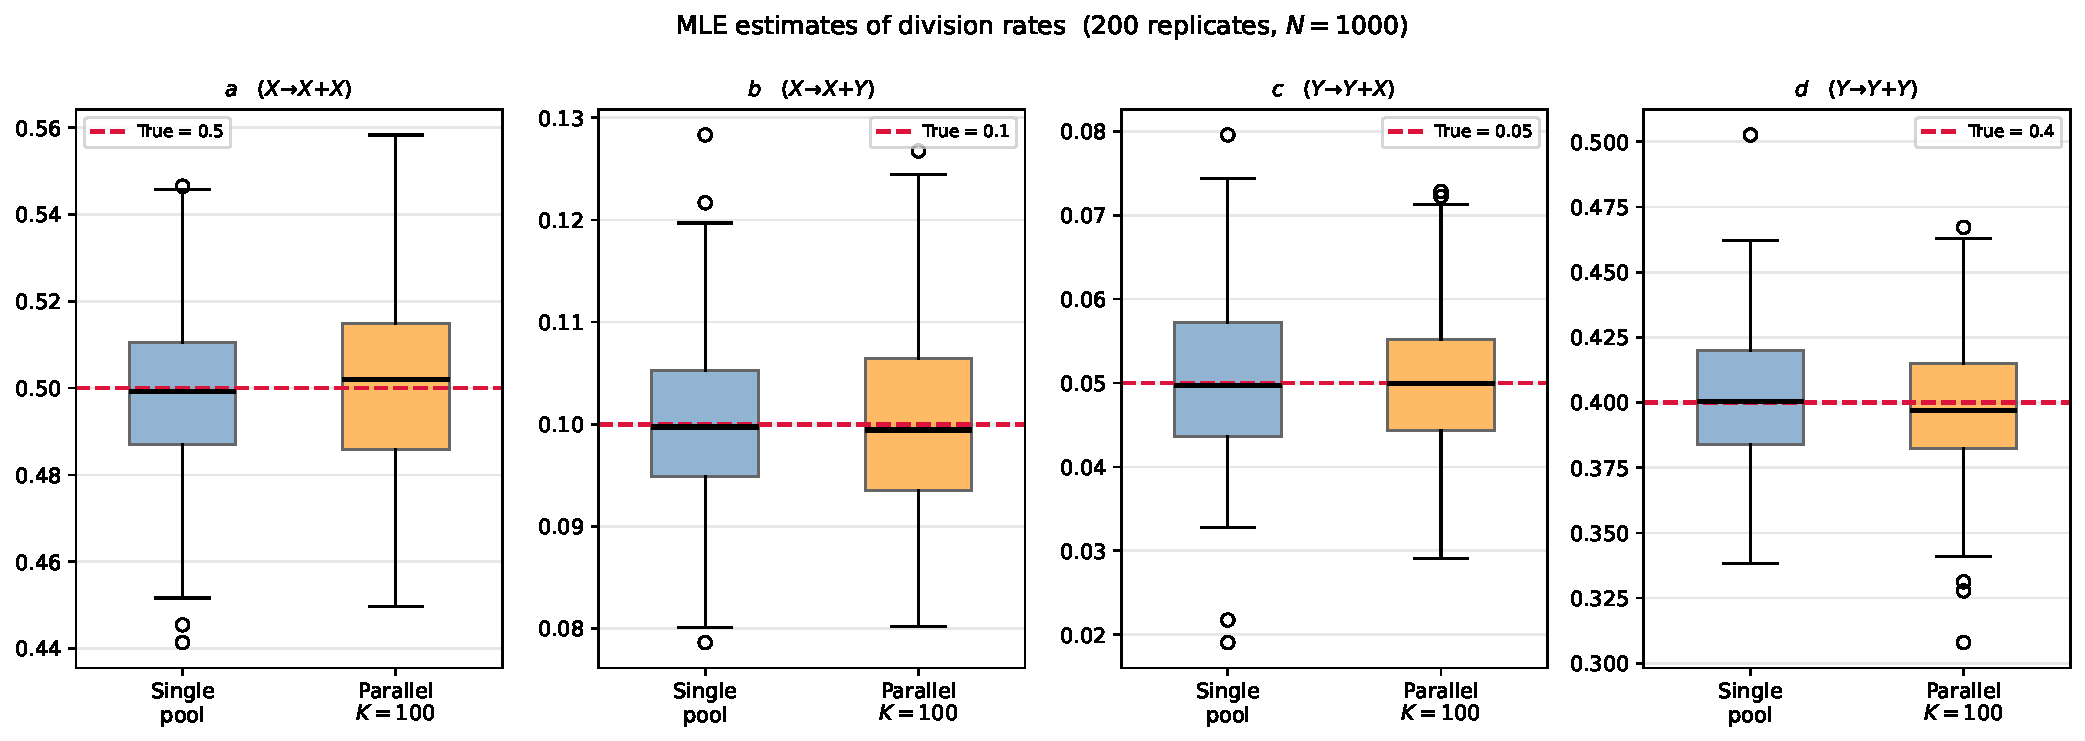
\includegraphics[width=\textwidth]{fig_estimation.pdf}
  \caption{Box plots of MLE estimates over $M = 200$ replicate simulations
           ($N = 1000$).  Blue boxes: single pool; orange boxes: parallel
           splitting ($K = 100$, $p = 0.5$).  Red dashed lines mark the
           true parameter values $a = 0.5$, $b = 0.1$, $c = 0.05$,
           $d = 0.4$.}
  \label{fig:estimation}
\end{figure}

Numerical results are summarized in Table~\ref{tab:estimation}.

\begin{table}[H]
\centering
\caption{MLE summary over $M = 200$ replicates, $N = 1000$.
         Parallel scenario: $K = 100$, $p = 0.5$.}
\label{tab:estimation}
\begin{tabular}{lcrrrrr}
\toprule
 & & \multicolumn{2}{c}{Single pool} & \multicolumn{2}{c}{Parallel ($K=100$)} \\
\cmidrule(lr){3-4}\cmidrule(lr){5-6}
Parameter & True & Mean & SD & Mean & SD \\
\midrule
$a$ & 0.500 & 0.499 & 0.020 & 0.500 & 0.022 \\
$b$ & 0.100 & 0.100 & 0.008 & 0.100 & 0.009 \\
$c$ & 0.050 & 0.050 & 0.010 & 0.050 & 0.009 \\
$d$ & 0.400 & 0.401 & 0.027 & 0.398 & 0.027 \\
\bottomrule
\end{tabular}
\end{table}

\subsection{Missing-data estimation: counts only}
\label{sec:counts_only}

In some experimental settings the division type of each event is not
observed; only the cell-count trajectories $n_X(t)$ and $n_Y(t)$ are
available.  At each event step the observable is which cell type was
produced, but not which parent type caused it:

\begin{itemize}
  \item \emph{X-producing step} ($n_X \to n_X+1$): event is
        $X\!\to\!X{+}X$ (rate $a n_X$) or $Y\!\to\!Y{+}X$ (rate $c n_Y$).
  \item \emph{Y-producing step} ($n_Y \to n_Y+1$): event is
        $X\!\to\!X{+}Y$ (rate $b n_X$) or $Y\!\to\!Y{+}Y$ (rate $d n_Y$).
\end{itemize}

The resulting \emph{incomplete-data log-likelihood} is obtained by
marginalising over the unobserved event labels:
\begin{equation}
  \ell_{\mathrm{obs}}(a,b,c,d)
  = \sum_{\text{X-steps}} \log(a n_X + c n_Y)
  + \sum_{\text{Y-steps}} \log(b n_X + d n_Y)
  - (a+b)\Lambda_X - (c+d)\Lambda_Y,
  \label{eq:ell_obs}
\end{equation}
where the sums are over the pre-event state at each step and
$\Lambda_X, \Lambda_Y$ are the same exposures as before (computed from
the observed trajectory).  The log-likelihood \eqref{eq:ell_obs} is
strictly concave and maximised by the system of score equations
\begin{equation}
  \sum_{\text{X-steps}} \frac{n_X}{a n_X + c n_Y} = \Lambda_X, \quad
  \sum_{\text{X-steps}} \frac{n_Y}{a n_X + c n_Y} = \Lambda_Y,
  \label{eq:score_obs}
\end{equation}
and analogously for $(b,d)$ from Y-producing steps.  These are solved by
L-BFGS-B with analytical gradients; starting values are obtained from the
unambiguous events (those where $n_Y = 0$, so $a$ and $b$ are fully
identifiable).

\paragraph{Near non-identifiability.}
The Fisher information matrix for $(a,c)$ from the incomplete-data
likelihood has elements
\[
  [I_{\mathrm{obs}}]_{ac}
  \propto \sum_{\text{X-steps}} \frac{n_X \, n_Y}{(a n_X + c n_Y)^2}.
\]
When the composition is near the equilibrium eigenvector
($n_X/n_Y \approx 1.37$), the matrix becomes nearly rank-one: any
parameter pair $(a',c')$ satisfying $a' n_X + c' n_Y \approx a n_X +
c n_Y$ (i.e.\ lying on the ``confusion ridge''
$a' + 1.37\,c' \approx \mathrm{const}$) yields approximately the same
likelihood.  Because the process spends most of its time near equilibrium,
the effective information about the individual rates $a$ and $c$ is far
smaller than in the complete-data case.  The same argument applies to
$(b,d)$.

\begin{figure}[H]
  \centering
  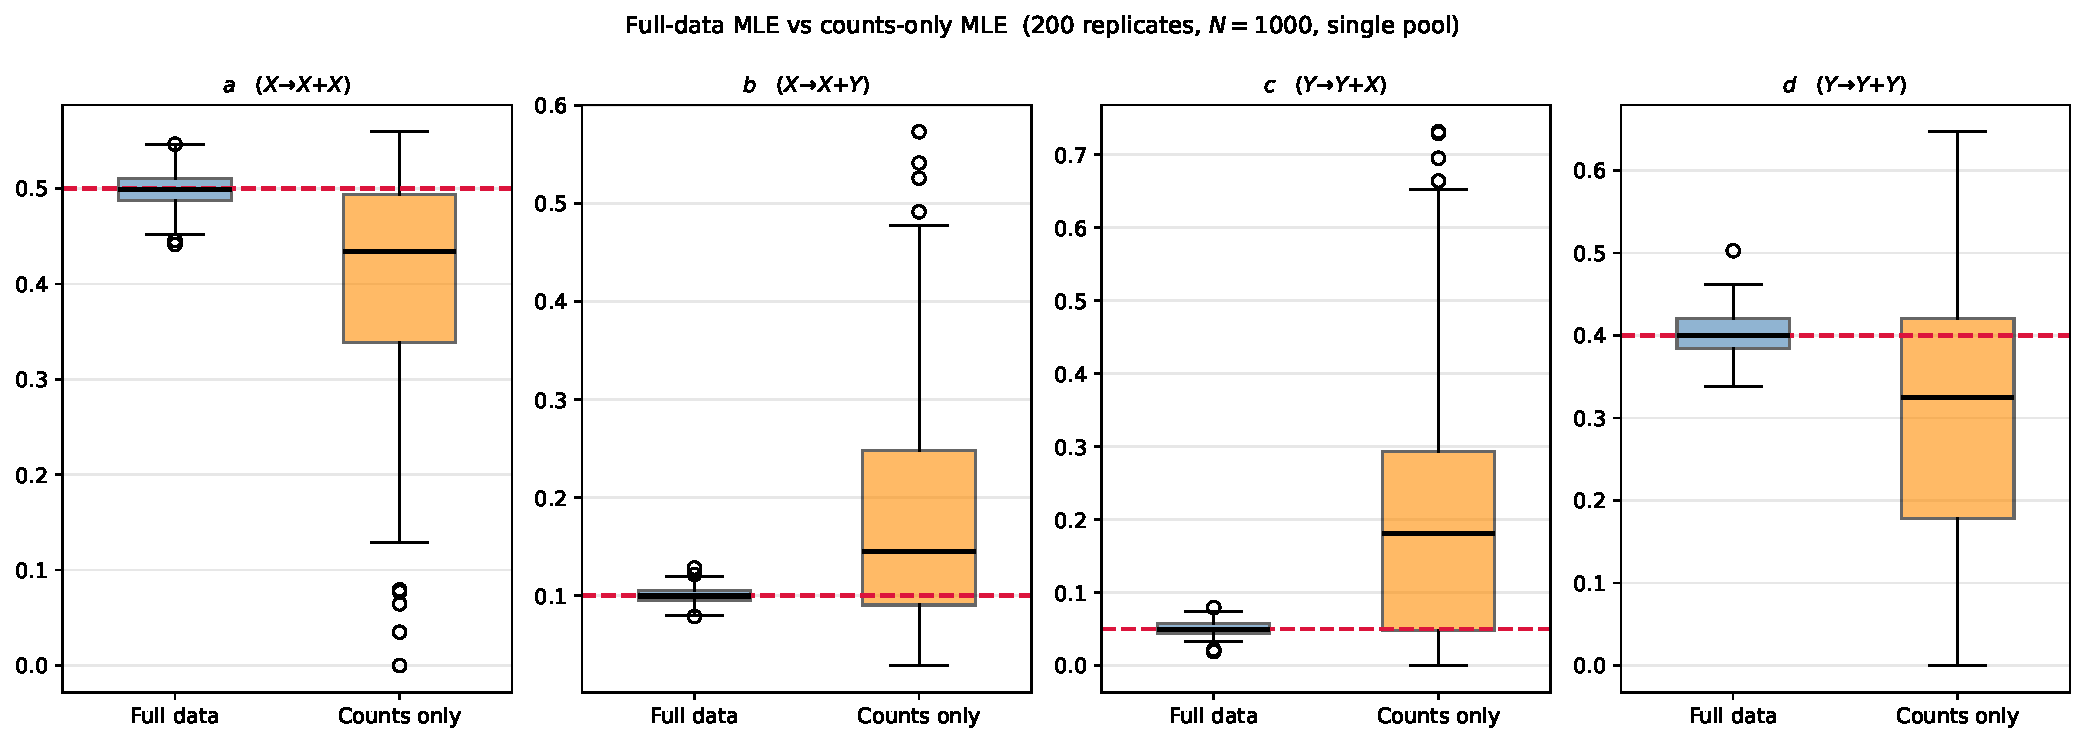
\includegraphics[width=\textwidth]{fig_estimation_counts.pdf}
  \caption{Full-data MLE (blue) vs counts-only MLE (orange) over
           $M = 200$ replicates ($N = 1000$, single pool).
           Red dashed lines mark the true values.
           The counts-only MLE is essentially unbiased but its standard
           deviation is $5$--$18\times$ larger than the full-data MLE
           due to near non-identifiability near the equilibrium composition.}
  \label{fig:est_counts}
\end{figure}

Table~\ref{tab:est_counts} quantifies the precision loss.  For $N=1000$
the counts-only SD exceeds the full-data SD by a factor of 6 for $a$
and $d$ and by a factor of 13--18 for $b$ and $c$ (the cross-production
rates, which are most susceptible to the confusion ridge).  Although the
estimator is consistent, the near non-identifiability means that very
large $N$ would be required to achieve practical accuracy.

\begin{table}[H]
\centering
\caption{MLE summary: full data vs counts-only ($M=200$, $N=1000$,
         single pool).}
\label{tab:est_counts}
\begin{tabular}{lcrrrr}
\toprule
 & & \multicolumn{2}{c}{Full-data MLE} & \multicolumn{2}{c}{Counts-only MLE} \\
\cmidrule(lr){3-4}\cmidrule(lr){5-6}
Parameter & True & Mean & SD & Mean & SD \\
\midrule
$a$ & 0.500 & 0.499 & 0.020 & 0.401 & 0.121 \\
$b$ & 0.100 & 0.100 & 0.008 & 0.183 & 0.116 \\
$c$ & 0.050 & 0.050 & 0.010 & 0.198 & 0.174 \\
$d$ & 0.400 & 0.401 & 0.027 & 0.296 & 0.166 \\
\bottomrule
\end{tabular}
\end{table}

The counts-only estimator is useful when no alternatives exist, but
Section~\ref{sec:first_event} shows that a simple change to the splitting
protocol can recover near full-data precision even without event labels.

\subsection{First-event estimation from single-cell seeding}
\label{sec:first_event}

\paragraph{Observation.}
When a pool is seeded with exactly \emph{one} cell the type of the first
division is unambiguously determined from the count increment alone:
\begin{itemize}
  \item \emph{X-seeded pool} ($n_X=1, n_Y=0$): only events
        $X\!\to\!X{+}X$ (rate $a$) and $X\!\to\!X{+}Y$ (rate $b$) are
        possible.  If $n_X$ increases, the event is type $a$; if $n_Y$
        increases, it is type $b$.
  \item \emph{Y-seeded pool} ($n_X=0, n_Y=1$): only events
        $Y\!\to\!Y{+}X$ (rate $c$) and $Y\!\to\!Y{+}Y$ (rate $d$) are
        possible, identifiable by the same count-change rule.
\end{itemize}
The seeding probability $p$ therefore determines which rates are
estimable: $p=0$ (all Y-seeded) gives information only on $c$ and $d$;
$p=1$ (all X-seeded) gives only $a$ and $b$.  For all four rates to be
estimable we need $p \in (0,1)$.

\paragraph{MLE with censoring.}
The time to the first event in an X-seeded pool is $\mathrm{Exp}(a+b)$,
and the event is type $a$ with probability $a/(a+b)$.  Not all pools
fire their first event before the simulation ends at $T_{\mathrm{stop}}$;
pools created late may be \emph{right-censored} at $T_{\mathrm{stop}} -
t_0$ (where $t_0$ is the pool-creation time).  The censored MLE is
\begin{equation}
  \hat{a} = \frac{n_a^{\mathrm{FE}}}{T_X}, \quad
  \hat{b} = \frac{n_b^{\mathrm{FE}}}{T_X},
  \label{eq:fe_mle}
\end{equation}
where $n_a^{\mathrm{FE}}$ counts the X-seeded pools whose first event
was type $a$, and
\[
  T_X = \sum_{\substack{i:\,\text{X-seeded},\\ \text{uncensored}}} t_{\mathrm{first},i}
      + \sum_{\substack{i:\,\text{X-seeded},\\ \text{censored}}} (T_{\mathrm{stop}} - t_{0,i}).
\]
Analogous formulae~\eqref{eq:fe_mle} apply to Y-seeded pools for $c$ and
$d$.  The estimator is consistent and approximately unbiased for any
choice of $K$ and $p \in (0,1)$.

\paragraph{Simulation results.}
Figure~\ref{fig:est_fe} and Table~\ref{tab:est_fe} compare the
first-event MLE (with $K = 20$, $p = 0.5$) against the full-data MLE.
With $N = 1000$ the first-event estimator is effectively unbiased and
has SDs $2$--$4\times$ larger than the full-data MLE — a dramatic
improvement over the counts-only estimator.

\begin{figure}[H]
  \centering
  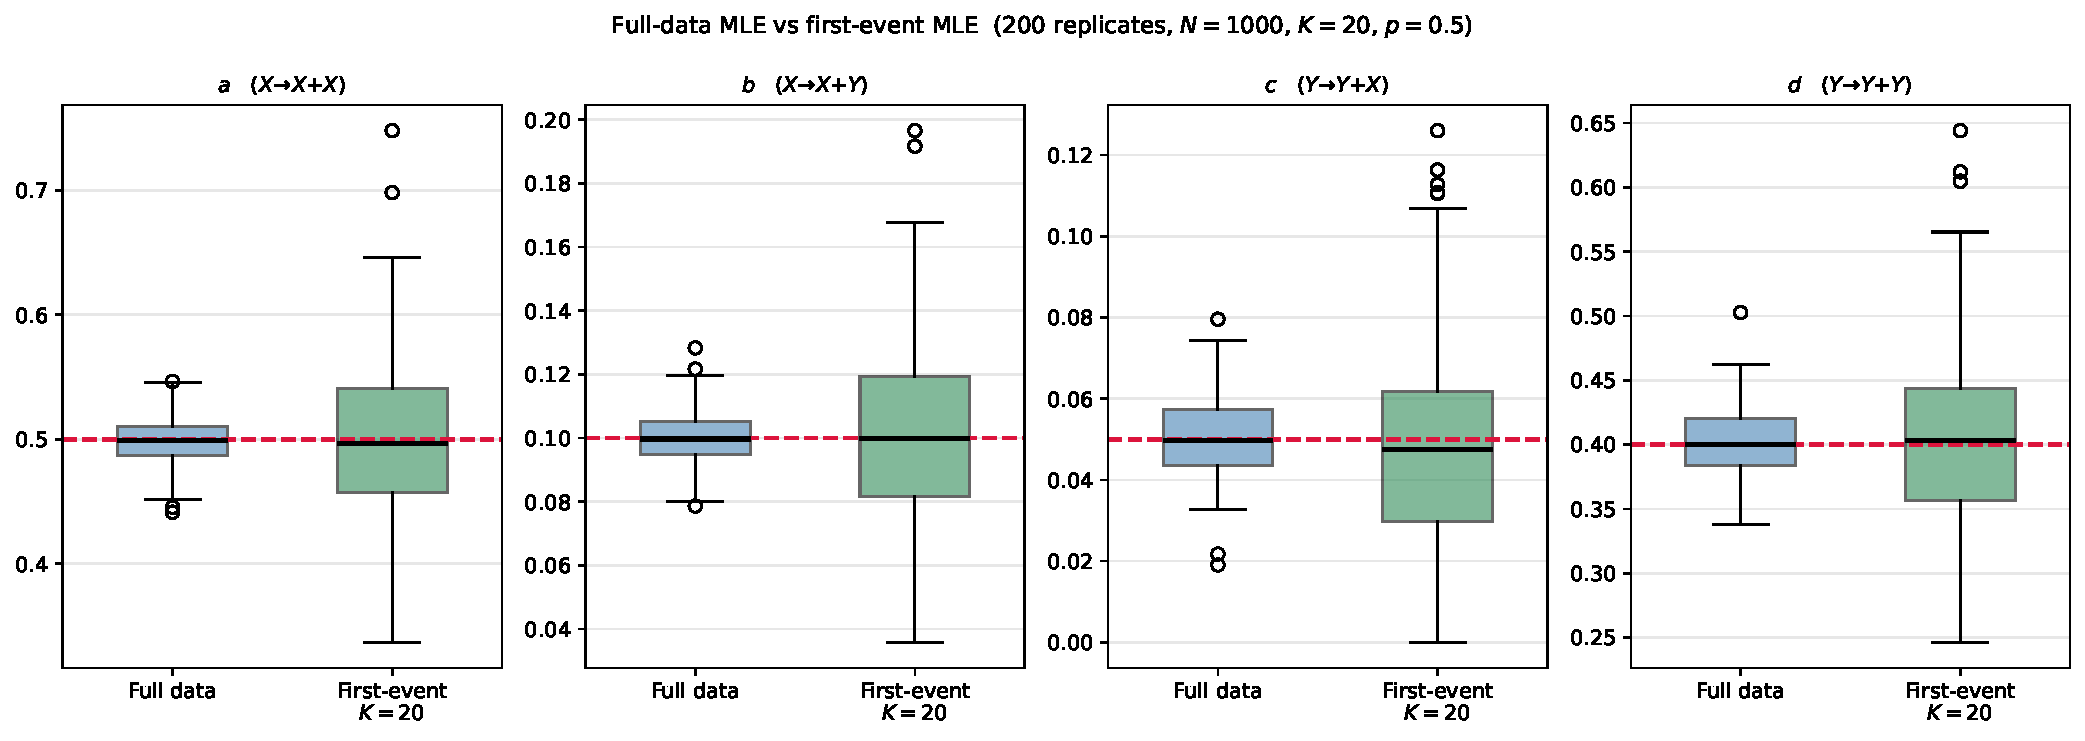
\includegraphics[width=\textwidth]{fig_estimation_first_event.pdf}
  \caption{Full-data MLE (blue) vs first-event MLE (green, $K = 20$,
           $p = 0.5$) over $M = 200$ replicates ($N = 1000$).  Red dashed
           lines mark the true values.  The first-event MLE is essentially
           unbiased and has $2$--$4\times$ the SD of the full-data MLE.}
  \label{fig:est_fe}
\end{figure}

\begin{table}[H]
\centering
\caption{First-event MLE summary ($M=200$, $N=1000$, $K=20$, $p=0.5$).}
\label{tab:est_fe}
\begin{tabular}{lcrrrr}
\toprule
 & & \multicolumn{2}{c}{Full-data MLE} & \multicolumn{2}{c}{First-event MLE} \\
\cmidrule(lr){3-4}\cmidrule(lr){5-6}
Parameter & True & Mean & SD & Mean & SD \\
\midrule
$a$ & 0.500 & 0.499 & 0.020 & 0.500 & 0.064 \\
$b$ & 0.100 & 0.100 & 0.008 & 0.102 & 0.030 \\
$c$ & 0.050 & 0.050 & 0.010 & 0.048 & 0.025 \\
$d$ & 0.400 & 0.401 & 0.027 & 0.407 & 0.067 \\
\bottomrule
\end{tabular}
\end{table}

\paragraph{Effect of pool size $K$: non-monotone behaviour and the $K=2$ case.}
The total number of child pools is \emph{not} a simple decreasing function of
$K$.  Because of the cascade dynamics described in Section~\ref{sec:comparison},
pool count has a \emph{minimum} near $K = 50$ and then \emph{rises again} for
larger $K$, before collapsing sharply near $K = N$ when few splits complete
before $T_{\mathrm{stop}}$ (Table~\ref{tab:fe_K}).  Since each single-cell child
pool contributes exactly one first-event observation, the SD of the first-event
estimator tracks this non-monotone pool count: it is smallest at $K = 2$,
reaches a local \emph{maximum} around $K = 50$, decreases to a local minimum
around $K = 200$, and then rises steeply as $K$ approaches $N$.

With $K = 2$ the cascade is maximal — virtually every division in the system
becomes the ``first event'' of some single-cell child pool — so the first-event
MLE \emph{observes essentially the same events as the full-data MLE}.  This
answers \textbf{Q1}: the gap at $K = 2$ relative to the full-data MLE is small
and arises solely from right-censoring of pools seeded near $T_{\mathrm{stop}}$
that do not fire before the simulation ends.

Figure~\ref{fig:fe_vs_K} confirms the non-monotone shape for $K$ swept from
$2$ to $900$ (\textbf{Q2}).  Table~\ref{tab:fe_K} also reports the expected
number of pools $E[\text{pools}]$ as a proxy for experimental cost, enabling
the cost--precision tradeoff discussed in Section~\ref{sec:cost_tradeoff}.

\begin{figure}[H]
  \centering
  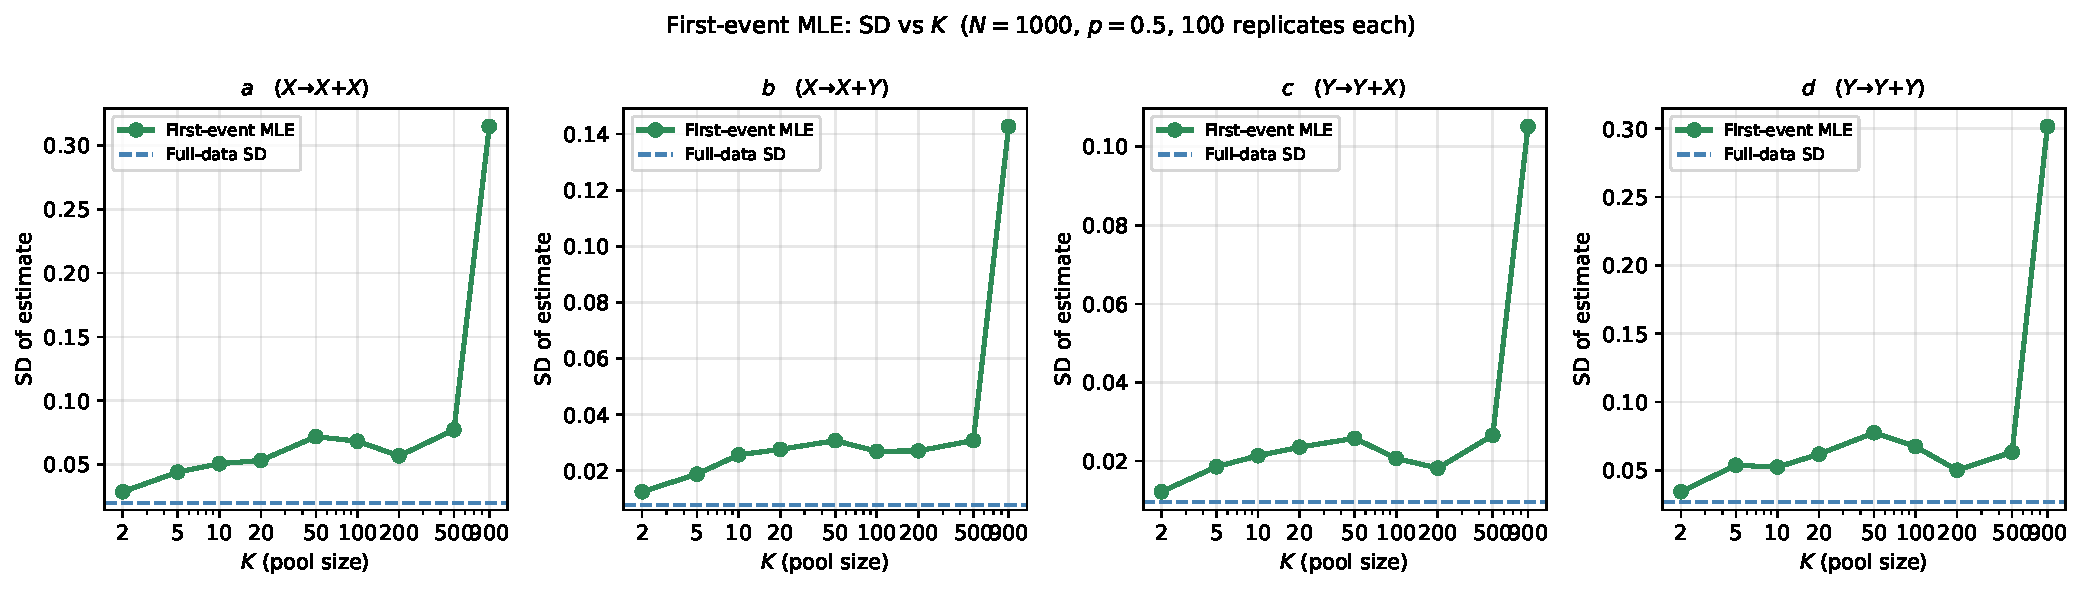
\includegraphics[width=\textwidth]{fig_first_event_vs_K.pdf}
  \caption{Standard deviation of the first-event MLE as a function of pool
           size $K$ ($N = 1000$, $p = 0.5$, 100 replicates per $K$, log
           $x$-axis).  Dashed lines show full-data MLE standard deviations.
           The curve is non-monotone: SD is lowest at $K = 2$ (many pools,
           nearly every division observed), reaches a local maximum near
           $K = 50$ (pool count is minimised by the cascade), dips again
           near $K = 200$, and then rises sharply as $K \to N$ (cascade
           collapses).}
  \label{fig:fe_vs_K}
\end{figure}

\begin{table}[H]
\centering
\caption{First-event MLE standard deviations and expected pool count as a
         function of $K$ ($N = 1000$, $p = 0.5$, 100 replicates per $K$).
         $E[\text{pools}]$ is the mean total number of pools generated;
         $E[q_X]$ and $E[q_Y]$ are the mean numbers of X- and Y-seeded
         single-cell child pools that contribute first-event observations.}
\label{tab:fe_K}
\begin{tabular}{rrrrrrrr}
\toprule
$K$ & SD($\hat{a}$) & SD($\hat{b}$) & SD($\hat{c}$) & SD($\hat{d}$)
    & $E[\text{pools}]$ & $E[q_X]$ & $E[q_Y]$ \\
\midrule
   2 & 0.029 & 0.013 & 0.012 & 0.034 & 1001 & 658 & 343 \\
   5 & 0.044 & 0.019 & 0.019 & 0.054 &  480 & 309 & 172 \\
  10 & 0.051 & 0.026 & 0.021 & 0.052 &  354 & 221 & 133 \\
  20 & 0.053 & 0.028 & 0.024 & 0.062 &  289 & 176 & 113 \\
  50 & 0.072 & 0.031 & 0.026 & 0.077 &  169 & 111 &  58 \\
 100 & 0.068 & 0.027 & 0.021 & 0.067 &  243 & 153 &  91 \\
 200 & 0.057 & 0.027 & 0.018 & 0.050 &  335 & 189 & 146 \\
 500 & 0.077 & 0.031 & 0.027 & 0.063 &  355 & 177 & 177 \\
 900 & 0.315 & 0.143 & 0.105 & 0.302 &   98 &  49 &  49 \\
\bottomrule
\end{tabular}
\end{table}

\subsection{Cost--precision tradeoff}
\label{sec:cost_tradeoff}

Each additional pool imposes an experimental cost (e.g.\ a culture well, a
sequencing lane).  A natural cost--efficiency metric is
\[
  \eta(K) = \frac{1}{\mathrm{SD}(\hat\theta)^2 \cdot E[\text{pools}]},
\]
which measures precision (Fisher information, approximately) per unit cost.
Table~\ref{tab:efficiency} reports $\eta(K)$ for each rate, normalised so that
$\eta(K=100) = 1$.

\begin{table}[H]
\centering
\caption{Relative efficiency $\eta(K)/\eta(K{=}100)$ of the first-event MLE
         for each rate parameter.  Values $>1$ mean more precision per pool
         than at $K = 100$.}
\label{tab:efficiency}
\begin{tabular}{rrrrrr}
\toprule
$K$ & $E[\text{pools}]$ & $\eta_a$ & $\eta_b$ & $\eta_c$ & $\eta_d$ \\
\midrule
   2 & 1001 & 1.38 & 1.13 & 0.70 & 0.94 \\
   5 &  480 & 1.22 & 1.04 & 0.63 & 0.80 \\
  10 &  354 & 1.25 & 0.76 & 0.64 & 1.14 \\
  20 &  289 & 1.38 & 0.80 & 0.65 & 1.00 \\
  50 &  169 & 1.30 & 1.10 & 0.93 & 1.09 \\
 100 &  243 & 1.00 & 1.00 & 1.00 & 1.00 \\
 200 &  335 & 1.05 & 0.72 & 0.94 & 1.31 \\
 500 &  355 & 0.54 & 0.53 & 0.41 & 0.78 \\
 900 &   98 & 0.12 & 0.09 & 0.10 & 0.12 \\
\bottomrule
\end{tabular}
\end{table}

The key findings are:
\begin{itemize}
  \item \textbf{The optimal $K$ depends on which rate is of primary interest.}
        $K = 2$ and $K = 20$ maximise efficiency for the X-cell rates $a$ (both
        give $\eta_a = 1.38$), while $K = 200$ maximises efficiency for the
        Y-cell rate $d$ ($\eta_d = 1.31$) and $K = 100$ is near-optimal for
        the rare cross-rate $c$.  There is no single $K$ that dominates for
        all four parameters.

  \item \textbf{The $q_X / q_Y$ imbalance explains the parameter-specific
        optima.}  At small $K$, many more X-seeded pools are created than
        Y-seeded pools (e.g.\ $q_X = 658$ vs $q_Y = 343$ at $K = 2$),
        because the pool composition at the time of splitting is biased
        toward type $X$ (the dominant type).  This gives disproportionately
        high precision for $a$ and $b$ but lower precision for $c$ and $d$.
        At larger $K$ (e.g.\ $K = 500$) the seedings become balanced
        ($q_X \approx q_Y$), which relatively favours Y-rate estimation.

  \item \textbf{$K = 50$ is the least efficient intermediate choice.}  It
        minimises the cascade pool count (Table~\ref{tab:fe_K}), delivering
        the worst combination of few observations and moderate imbalance.

  \item \textbf{$K > 200$ rapidly loses efficiency.}  By $K = 500$ all
        efficiencies drop below 0.8 relative to $K = 100$, and $K = 900$
        is essentially uninformative ($\eta < 0.12$ for all parameters).
\end{itemize}

\subsection{Conclusions}

\begin{enumerate}
  \item \textbf{Both estimators are effectively unbiased.}
        The simulation means in Table~\ref{tab:estimation} differ from the
        true values by less than $0.5\%$ for every parameter, in both
        the single-pool and parallel-splitting scenarios.

  \item \textbf{Standard deviations are comparable across scenarios.}
        The two scenarios achieve similar estimation precision at the same
        $N$.  The parallel case has marginally larger SD for $a$ and $b$
        (the $X$-cell rates), reflecting the smaller effective exposure
        per pool, but marginally smaller SD for $c$ (the $Y\!\to\!Y{+}X$
        rate), because averaging across many pools stabilizes the count
        of rare events.

  \item \textbf{Rates involving $Y$ cells ($c$ and $d$) are estimated with
        relatively higher coefficient of variation (CV).}
        Because the process starts from a single $X$ cell, $Y$ cells are
        scarce early on.  The $Y$-cell exposure $\Lambda_Y$ is therefore
        smaller than $\Lambda_X$, yielding larger relative uncertainty in
        $c$ and $d$.  Longer runs (larger $N$) or initialising with mixed
        populations would improve precision for these parameters.

  \item \textbf{The tail correction is essential for parallel splitting.}
        Without it, rates are overestimated by $20$--$30\%$ because the
        missing interval $[t^{(p)}_{\mathrm{last}}, T_{\mathrm{stop}}]$ is
        not counted in the exposure.  After the correction both estimators
        have comparable performance (Table~\ref{tab:estimation}).

  \item \textbf{Consistency.}  Simulations at $N = 5\,000$ and
        $N = 20\,000$ (not shown) confirm that both estimators converge to
        the true values as $N$ increases, consistent with the general
        theory of MLE for CTMCs~\cite{athreya1972}.

  \item \textbf{When only counts are observable, near non-identifiability
        severely inflates variance.}
        The counts-only MLE (Section~\ref{sec:counts_only}) is consistent
        but its SD at $N = 1000$ is $6$--$18\times$ larger than the
        full-data MLE.  The near non-identifiability arises because the
        process spends most of its time near the equilibrium composition,
        where $a n_X + c n_Y$ is approximately proportional to $n_X$,
        making $a$ and $c$ nearly confounded.

  \item \textbf{Single-cell seeding restores near full-data precision.}
        The first-event MLE (Section~\ref{sec:first_event}) exploits the
        fact that a pool seeded with one cell has unambiguous event types
        at its first division.  With $K = 20$ and $p = 0.5$ it achieves
        SDs only $2$--$4\times$ larger than the full-data MLE (versus
        $6$--$18\times$ for counts only), with no additional experimental
        data beyond the count trajectories.  Smaller $K$ further reduces
        variance by creating more pools (Figure~\ref{fig:fe_vs_K}).
        The seeding probability $p$ must satisfy $0 < p < 1$; choosing
        $p = 0$ or $p = 1$ makes two of the four rates unestimable from
        first events.
\end{enumerate}


% ─────────────────────────────────────────────────────────────────────────────
\section{Pure-Pool Splitting: a Multi-Cell First-Event Scheme}
\label{sec:pure_pool}

\subsection{Motivation}

In the single-cell first-event scheme (Section~\ref{sec:first_event}) each
child pool starts from exactly one founder cell and contributes a single binary
observation — effectively a $\mathrm{Binomial}(1,\,p)$ trial — to the
estimation of $p = a/(a+b)$ (for X-seeded pools) or $q = c/(c+d)$ (for
Y-seeded pools).  The information per pool is therefore low: regardless of how
many cells the pool eventually contains, the observation reduces to a single
coin flip about $p$.

The \emph{pure-pool} scheme breaks this constraint by running each pure pool
until the first cross-type event rather than stopping after one trial.  The
number of same-type events observed before that termination is itself
informative about $p$, converting the per-pool data structure from a
$\mathrm{Binomial}(1,p)$ experiment to a
$\mathrm{NegativeBinomial}(1,\,1-p)$ (equivalently,
$\mathrm{Geometric}(1-p)$) experiment.

Concretely, this is achieved by replacing single-cell founders with entire
pure populations.  When any pool first satisfies $\min(n_X,\,n_Y) \ge K$, it
is dissolved and replaced by two \emph{pure} pools:
\begin{itemize}
  \item a \textbf{pure-X pool} containing all $n_X$ cells of type $X$ (and
        0 cells of type $Y$), and
  \item a \textbf{pure-Y pool} containing all $n_Y$ cells of type $Y$.
\end{itemize}
Each pure pool then evolves independently.  Because a pure-X pool has no
$Y$ cells, every division event is unambiguously type $a$ ($X\!\to\!X{+}X$)
or type $b$ ($X\!\to\!X{+}Y$): the event type is fully determined by
the count change alone, without requiring individual event labels.  The
\emph{pure phase} lasts until the first cross-type event
($X\!\to\!X{+}Y$ for a pure-X pool), after which the pool returns to mixed
status and may eventually trigger a new split.

\subsection{Information gain per pool}

In a pure-X pool, successive events are independent Bernoulli trials with
$P(\text{type }a) = a/(a+b)$, regardless of the current pool size (the pool
size cancels from the competing rates $a\,n_X$ and $b\,n_X$).  The pure phase
ends at the first type-$b$ event, so the number of type-$a$ events
$k_a \sim \mathrm{Geometric}(b/(a+b))$ with mean $(a+b)/b$.  For our
parameters,
\[
  E[\text{events per pure-X pool}] = \frac{a+b}{b} = \frac{0.6}{0.1} = 6,
  \qquad
  E[\text{events per pure-Y pool}] = \frac{c+d}{c} = \frac{0.45}{0.05} = 9.
\]

The pure-pool MLE benefits from \emph{two} distinct information sources that
are absent in the single-cell scheme.
\begin{enumerate}
  \item \textbf{Count information (Negative Binomial).}  The ratio
        $k_a / (k_a + 1)$ is a consistent estimate of $p = a/(a+b)$
        derived entirely from event counts, with no need for timing.
        This is the sufficient statistic of the
        $\mathrm{NegBin}(1,\,b/(a+b))$ model.  In the single-cell scheme
        $k_a \in \{0,1\}$ and this ratio equals the single binary outcome —
        no richer than one coin flip.
  \item \textbf{Timing information (Poisson process).}  The integrated
        exposure $\Lambda_X$ and the total event count $k_a + 1$ jointly
        estimate the overall rate $a + b$, exactly as in the standard CTMC
        MLE.
\end{enumerate}
The combined MLE $\hat a = n_a/\Lambda_X$ uses both sources simultaneously.
The Fisher information about $p_X = a/(a+b)$ per pool is therefore
$\approx (a+b)/b = 6$ times larger than in the single-cell scheme
(which always contributes exactly one Bernoulli trial).

\subsection{Estimator}

The likelihood in the pure phase factors as in Section~\ref{sec:estimation}.
For all pure-X pools combined, the sufficient statistics are the total
type-$a$ event count $n_a^{\mathrm{PP}}$, the total type-$b$ event count
$n_b^{\mathrm{PP}}$ (one per pool that completes its pure phase), and the
total X-cell exposure $\Lambda_X^{\mathrm{PP}} = \sum_p \int n_X^{(p)}(t)\,dt$
over all pure-X phases.  The MLE is identical in form to~\eqref{eq:mle}:
\begin{equation}
  \hat{a} = \frac{n_a^{\mathrm{PP}}}{\Lambda_X^{\mathrm{PP}}},\quad
  \hat{b} = \frac{n_b^{\mathrm{PP}}}{\Lambda_X^{\mathrm{PP}}},\quad
  \hat{c} = \frac{n_c^{\mathrm{PP}}}{\Lambda_Y^{\mathrm{PP}}},\quad
  \hat{d} = \frac{n_d^{\mathrm{PP}}}{\Lambda_Y^{\mathrm{PP}}}.
  \label{eq:mle_pp}
\end{equation}

\subsection{Simulation study and cost comparison}

Table~\ref{tab:pure_pool} and Figure~\ref{fig:pure_pool_K10} compare the
pure-pool MLE against the single-cell first-event MLE and the full-data
MLE for $K = 10$ and $N = 1000$ over $M = 200$ replicates.

\begin{table}[H]
\centering
\caption{MLE comparison at $N=1000$, $M=200$ replicates.
         ``FE'' = single-cell first-event ($p=0.5$);
         ``PP'' = pure-pool.  The mean number of pure pools generated
         is 30 (FE: 355 single-cell pools) for $K=10$,
         and 7 (FE: 170) for $K=50$.}
\label{tab:pure_pool}
\begin{tabular}{lcrrrrrr}
\toprule
 & & & \multicolumn{2}{c}{First-event ($K$)} &
         \multicolumn{2}{c}{Pure-pool ($K$)} \\
\cmidrule(lr){4-5}\cmidrule(lr){6-7}
Param & True & Full-data SD & Mean & SD & Mean & SD \\
\midrule
\multicolumn{7}{l}{\emph{$K = 10$}} \\
$a$ & 0.500 & 0.020 & 0.511 & 0.053 & 0.516 & 0.063 \\
$b$ & 0.100 & 0.008 & 0.103 & 0.022 & 0.108 & 0.027 \\
$c$ & 0.050 & 0.010 & 0.050 & 0.020 & 0.057 & 0.020 \\
$d$ & 0.400 & 0.027 & 0.401 & 0.057 & 0.428 & 0.052 \\
\addlinespace
\multicolumn{7}{l}{\emph{$K = 50$}} \\
$a$ & 0.500 & 0.020 & 0.505 & 0.069 & 0.520 & 0.141 \\
$b$ & 0.100 & 0.008 & 0.102 & 0.030 & 0.142 & 0.116 \\
$c$ & 0.050 & 0.010 & 0.050 & 0.025 & 0.080 & 0.081 \\
$d$ & 0.400 & 0.027 & 0.410 & 0.075 & 0.411 & 0.108 \\
\bottomrule
\end{tabular}
\end{table}

\begin{figure}[H]
  \centering
  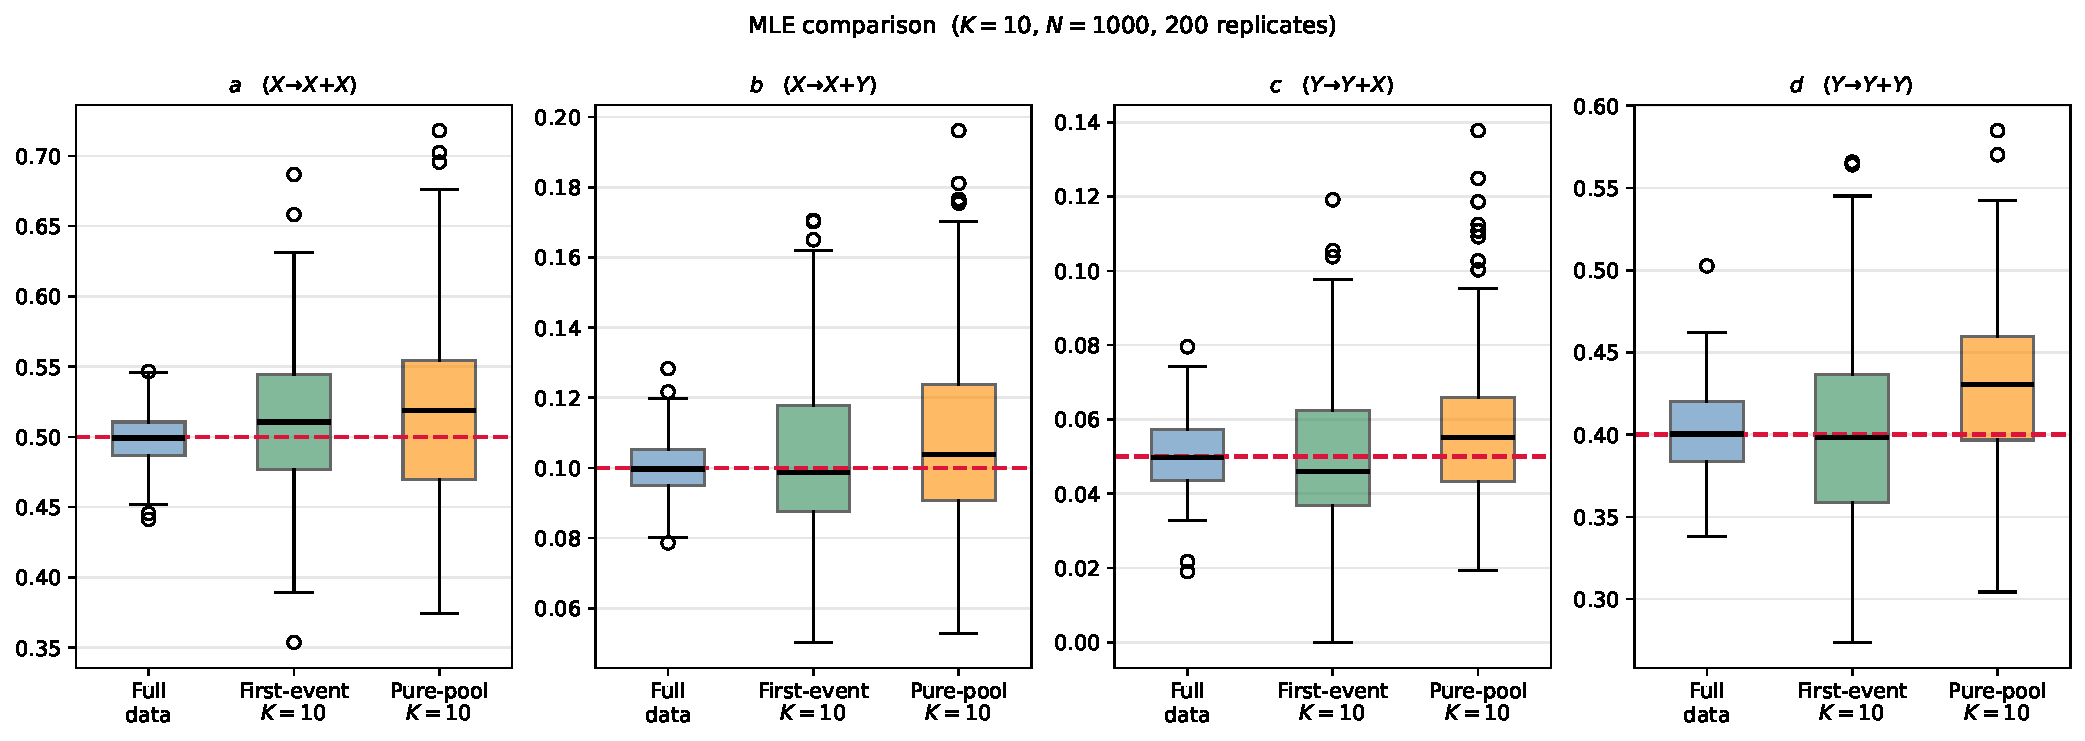
\includegraphics[width=\textwidth]{fig_pure_pool_K10.pdf}
  \caption{MLE comparison at $K = 10$, $N = 1000$, $M = 200$ replicates.
           Blue: full-data MLE (benchmark).  Green: single-cell first-event
           MLE ($K=10$, $p=0.5$, 355 single-cell pools).  Orange: pure-pool
           MLE ($K=10$, 30 pure pools).  Red dashed lines: true values.}
  \label{fig:pure_pool_K10}
\end{figure}

\subsection{Conclusions}

\begin{itemize}
  \item \textbf{At fixed $N$, single-cell first-event outperforms pure-pool.}
        Table~\ref{tab:pure_pool} shows that for $K = 10$ and $N = 1000$,
        the single-cell first-event MLE has lower SD than the pure-pool MLE
        for three of four parameters ($a$, $b$, $d$).  The reason is simple:
        the $\min(X,Y) \ge K$ trigger is harder to satisfy than total
        cells $= K$, so it fires far less often — generating only $\approx 30$
        pure pools vs.\ $\approx 355$ single-cell pools.  Fewer pools
        dominate even though each pure pool is individually more informative.

  \item \textbf{Each pure pool carries more information per split event.}
        In a pure-X pool every event is an unambiguous Bernoulli$(a/(a+b))$
        trial; the pure phase lasts $(a+b)/b \approx 6$ events on average.
        This is $\approx 6\times$ the information of a single-cell pool
        (one trial).  If the \emph{number of split events} (e.g.\ experimental
        passages) is the binding cost rather than total cell count, the
        pure-pool scheme is preferable: it extracts more information from
        each split.

  \item \textbf{Large $K$ is inadvisable.}
        At $K = 50$ only $\approx 7$ pure pools are generated at $N = 1000$,
        giving substantially higher variance and noticeable finite-sample
        bias (see the $K=50$ block of Table~\ref{tab:pure_pool}).
        Small $K$ (e.g.\ $K = 5$--$10$) is recommended for the pure-pool
        scheme.
\end{itemize}

% ─────────────────────────────────────────────────────────────────────────────
\section{Discussion}
\label{sec:discussion}

\subsection{Founder effect and bottlenecks}

The dominant feature of the splitting simulation is a manifestation of the
\emph{founder effect}: when a new pool is established from a single individual,
the type of the founder disproportionately shapes the descendant population.
With $K = 100$ this effect is weak, because each pool grows long enough for
the composition to approach the eigenvector equilibrium before the next split.
In the parallel setting, coexistence of many pools at every instant further
averages out individual founder biases.

\subsection{Invariance of growth rate}

Because splits only redistribute existing cells (no net creation or
destruction), the dominant eigenvalue $\lambda_1$ and therefore the
exponential growth rate of the total population are the same in all
scenarios.  What changes is how quickly the composition vector $(X, Y)/N$
approaches the Perron eigenvector $\approx (0.578, 0.422)$.

\subsection{Practical interpretation}

If this model represents, for example, stem-cell passage in a culture dish,
the splitting threshold $K$ is the passage size and $p$ is the fraction of
stem cells (type $X$) deliberately maintained during passaging.  The analysis
shows that:
\begin{itemize}
  \item Passaging at a large $K$ is more ``self-correcting'' — the culture
        naturally drifts toward equilibrium composition.
  \item Parallel passaging (growing multiple sub-cultures simultaneously)
        greatly suppresses composition drift and renders the result nearly
        independent of the seeding protocol.
  \item Rate parameters $a$, $b$, $c$, $d$ can be estimated from the
        cell-count trajectory by the closed-form MLEs~\eqref{eq:mle},
        without requiring any additional experimental interventions.
        The estimators are practically unbiased and have comparable
        precision under both protocols for $N = 1000$ cells observed.
\end{itemize}


\begin{thebibliography}{9}

\bibitem{gillespie1977}
Gillespie, D.\,T.\ (1977).
Exact stochastic simulation of coupled chemical reactions.
\textit{The Journal of Physical Chemistry}, \textbf{81}(25), 2340--2361.
\url{https://doi.org/10.1021/j100540a008}

\bibitem{kesten1966}
Kesten, H.\ and Stigum, B.\,P.\ (1966).
A limit theorem for multidimensional Galton-Watson processes.
\textit{Annals of Mathematical Statistics}, \textbf{37}(5), 1211--1223.
\url{https://doi.org/10.1214/aoms/1177699266}

\bibitem{athreya1972}
Athreya, K.\,B.\ and Ney, P.\,E.\ (1972).
\textit{Branching Processes}.
Springer, Berlin.
\url{https://doi.org/10.1007/978-3-642-65371-1}

\bibitem{gillespie1976}
Gillespie, D.\,T.\ (1976).
A general method for numerically simulating the stochastic time evolution
of coupled chemical reactions.
\textit{Journal of Computational Physics}, \textbf{22}(4), 403--434.
\url{https://doi.org/10.1016/0021-9991(76)90041-3}

\end{thebibliography}

\end{document}
